% Figure blocks for the vardictcpp paper. The figures carry no title or in-figure prose;
% all descriptive text is in these captions. PDFs are produced by make_paper_assets.py.

\begin{figure}[t]
  \centering
  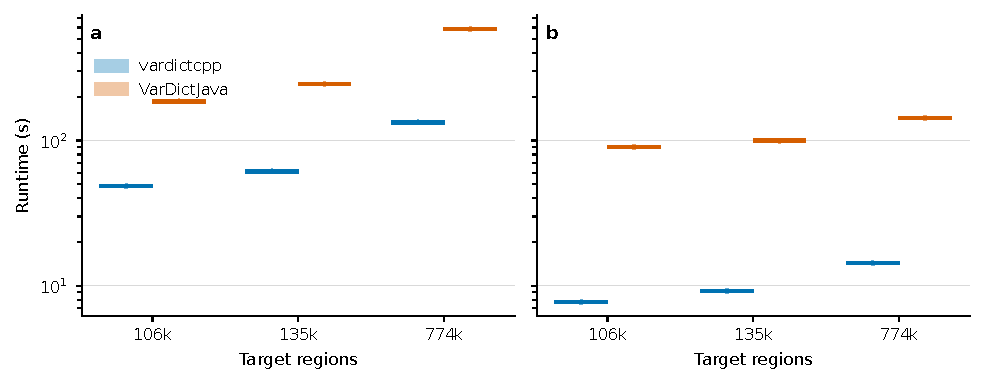
\includegraphics[width=\linewidth]{figures/fig1_runtime.pdf}
  \caption{\label{fig:runtime}%
    Wall-clock runtime of \textbf{vardictcpp} (blue) and \textbf{VarDict-Java 1.8.3} (orange) on three
    whole-exome samples at (\textbf{a}) one thread and (\textbf{b}) eight threads. Samples are labelled
    by target-region count on the $x$-axis: \texttt{SRR15006376} ($\sim$106\,k regions),
    \texttt{SRR15006540} ($\sim$135\,k), and \texttt{SRR8657348} ($\sim$774\,k, a high-coverage CCLE
    run). All runs used hg19, minimum allele frequency $0.01$, CPU affinity pinning, and were timed with
    \texttt{/usr/bin/time -v}; VarDictJava ran on JDK~25 with \texttt{-Xmx\,8g}. The $y$-axis is
    log-scaled; lower is faster. vardictcpp is $\sim$3.8--4.4$\times$ faster single-core and
    $\sim$10--12$\times$ faster at eight threads.}
\end{figure}

\begin{figure}[t]
  \centering
  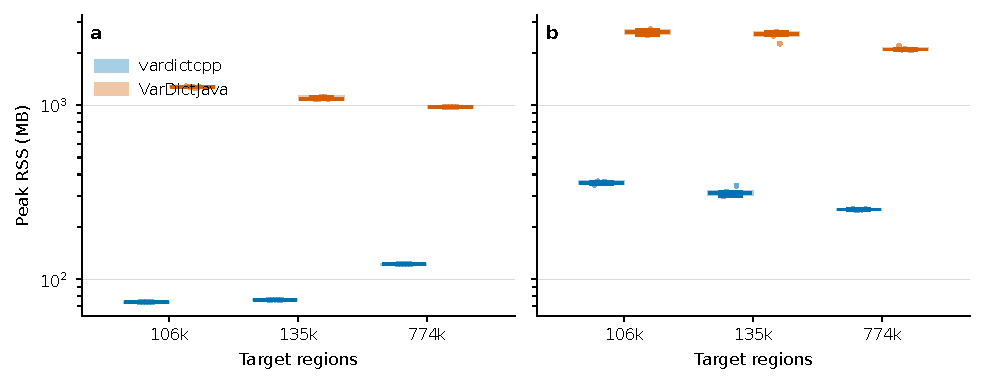
\includegraphics[width=\linewidth]{figures/fig2_memory.pdf}
  \caption{\label{fig:memory}%
    Peak resident set size (RSS) of \textbf{vardictcpp} (blue) and \textbf{VarDict-Java 1.8.3} (orange)
    on the same three samples at (\textbf{a}) one and (\textbf{b}) eight threads, same run configuration
    as Fig.~\ref{fig:runtime}. The $y$-axis is log-scaled (MB); lower is leaner. Single-threaded,
    vardictcpp holds 74--122\,MB against VarDictJava's $\sim$1.0--1.3\,GB (an $\sim$8--17$\times$
    reduction); at eight threads vardictcpp stays at 248--364\,MB against $\sim$2.1--2.7\,GB
    ($\sim$7--9$\times$). vardictcpp stores the reference as disjoint windows matching Java's
    reference map, so a distant realignment breakpoint never gap-fills a multi-megabase span.}
\end{figure}
